\documentclass{article}

\usepackage[utf8]{inputenc}
\usepackage{graphicx}

\graphicspath{ {imagens/} }
\title{Aulas de Estruturas de Dados e algoritmos 2}
\author{cotrim149}

\begin{document}
\maketitle

\section{Busca Sequencial}
	\begin{enumerate}
	\item Complexidade média(Tempo de demora para resposta): 
		\begin{equation}
		\frac{n}{2}			
		\end{equation}
	\item O(n)
	\item Métodos para otimização
		\begin{itemize}
		\item Sentinela: Consiste em adicionar um elemento de valor x no final do vetor.
		\end{itemize}		 
	\item Alternativa: Lista encadeada
	\item Aumento de eficiência
		\begin{itemize}
		\item Método mover para frente: Sempre que uma pesquisa obter êxito, o registro recuperado é colocado no ínicio da lista. \textbf{Desvantagem:} Qualquer informação fica privelegiada
		\item Método da transposição: Um registro recuperado com sucesso é trocado imediatamento com o elemento anterior (swap é O(1), não importando a quantidade de elementos). \textbf{Desvantagem:} Cancelamento da otimização, (swap alternados entre mesmos elementos)		
		\end{itemize}
	\item Tabela Ordenada
		\begin{itemize}
		\item Complexidade: O(n/2). \textbf{Pior caso:} Complexidade: O(n)
		\item Dificuldade: Manter tabela ordenada e a ordenação em si
		\end{itemize}
	\item Tabela indexada
		\begin{itemize}
		\item Utilização de tabela auxiliar como tabela de índices
		\item Cada elemento na tabela de índices contém uma chave (kindex) e um indicador do registro no arquivo que corresponde a kindex
		\end{itemize}
	\item Vantagens e desvantagens na busca sequêncial
		\begin{itemize}
		\item Vantagens: Os ítens poderão ser examinados sem serem acessados, o tempo de busca diminui consideravelmente
		\item Desvantagens: Tabela tenha que estar ordenada, demanda mais espaço.
		\end{itemize}
	\item Remoção
		\begin{itemize}
		\item Remova-se o elemento e rearranja-se a tabela
		\item Indicar que o local está vazio, e futuramente é inserido outro elemento no índice
		\end{itemize}
	\item Inserção
		\begin{itemize}
		\item Se houver espaço vago, rearranjam-se os elementos localmente, caso não haja espaço, toda a tabela deve ser rearranjada
		\end{itemize}
	\end{enumerate}
\section{Busca Binária}
	\begin{itemize}
	\item O(log n); Cada comparação reduz o número de possíveis candidatos por um fator de 2.
	\item Pode ser usada como organização de tabela sequencial indexada
	\item Desvantagem: Precisa de índices, não funciona em uma lista encadeada ou duplamente encadeada
	\end{itemize}

\section{Busca por interpolação}
	\begin{itemize}
	\item As chaves precisam estar uniformemente distribuidas
	
	\begin{equation}
		meio = inf + (sup - inf) * \frac{(x- A[inf])}{(A[sup]-A[inf])}
	\end{equation}		
	
	\item O(log(log(n))) se as chaves estiverem uniformemente distribuida
	\item Se chaves não estiverem uniformemente distribuidas, a busca por interpolação pode ser tão ruim quanto uma busca sequencial
	\item Desvantagem: 	Em situações práticas, as chaves tendem a se aglomerar em torno de determinados valores e não são uniformemente distribuidas
	\end{itemize}

\section{Busca em árvore}


	\begin{enumerate}

	\item pré-ordem (sempre a esquerda): [8,3,1,6,4,7,10,14,13]
	\item in-ordem (sempra em baixo): [1,3,4,6,7,8,10,13,14]
	\item pós-ordem (sempra a direita) : [1,4,7,6,3,13,14,10,8]

	\begin{figure}
		\centering	
		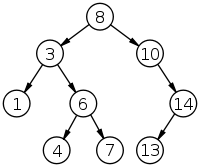
\includegraphics[scale=1]{arvorebinaria.jpg}
		\caption{Imagine uma linha passando sempre a esquerda de cada valor começando pela raiz} 	
	\end{figure}


	\end{enumerate}

\section{Selection Sort}
	\begin{itemize}
	\item Chamado de algoritmo natural
	\item Se baseia em passar o menor valor do vetor para a primeira posição
	\item complexidade média = (n-1)*(n/2)
	\item O(n2)	
	\end{itemize}
\section{Insertion Sort}
	\begin{itemize}
	\item Chamado de algoritmo natural
	\item Não existe swap para fora do vetor, sempre acrescente o "procurado" entre os valores
	\item 
		\begin{equation}
			complexidadeMedia = (n)*(\frac{n}{4})
		\end{equation}
		
		\begin{equation}
			Complexidade= O(n^{2})
		\end{equation}
	\end{itemize}
\section{Bubble sort}
	\begin{equation}
		Complexidade= O(n^{2})
	\end{equation}
	
\section{Shell sort}

	\begin{itemize}
	\item O mais eficiente algoritmo de ordenação dentre os de complexidade quadrática
	\item "Gaps" de n/2, sempre fazer o arrendondamento para baixo.
	\item Vizinho é igual a um "gap" de distância
	\item Refinamento do insertion Sort
	\item subvetores dentro do vetor(ideia!), subvetor com tamanho n/"gap"		
	
		\begin{equation}
			Complexidade= O(n^{2})
		\end{equation}

	\end{itemize}
	\begin{figure}
		\centering
		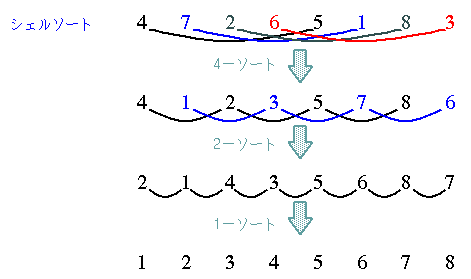
\includegraphics[trim = 35mm 2mm 2mm 2mm,clip]{shell-sort.png}
		\caption{\textbf{Shell Sort} Linha 1: Gap de n=4 com 4 subvetores; Linha 2: Gap de n=2 com 2 subvetores; Linha 3: Gap de n=1 com 1 subvetor, Linha 4: Ordenação completa}
	\end{figure}
	
	
	
\section{Bucket Sort}
	\begin{itemize}
	\item "Dividir e conquistar"
	\item Divisão em "baldes" por faixas de valores,
	\item pode ser usado qualquer algortimo dentro de cada balde
	\end{itemize}
	
\section{Quick Sort}
	\begin{itemize}
	\item "Dividir e conquistar"
	\item Escolhe-se um valor pivô e move-se todos os valores menores para a esquerda e os maiores para a direita
	\item Ordena-se recursivamente os valores menores e maiores
	\item Algoritmo instável: Não garante que elementos iguais não invertam, não se preocupa com a ordem dos elementos
	\item O(log(n))
	\item Desvantagem: A escolha de um mau pivô seguidamente podem tornar o algoritmo O(n2)
	\item Encontrar o mediano é O(n), o que resulta O(n log(n) ) 
	\item Algoritmo recursivo
	\end{itemize}

\section{Merge Sort}
	\begin{itemize}
	\item Algoritmo é recursivo, mas pode ser iterativo, existem mudanças de funcionamento.
	\item O(n log(n))
	\end{itemize}
\end{document}